\scanpage{50}
biextension \deleted{\unsure{de}} de $P,Q$ par $G$, et où $(E',\varphi)$ est le couple d'une biext. $E'$ de $P',Q$ par $G$ et d'un hom
\diagram{\begin{tikzcd}[ampersand replacement=\&]\varphi:T_{\mathbb P}(P)\times T_{\mathbb P}(Q)\arrow[r]\&T_{\mathbb P}(G)\end{tikzcd}}
\uline{qui étend l'hom}
\diagram{\begin{tikzcd}[ampersand replacement=\&]\deleted{\unsure{\varphi}}\ \varphi_{\mathbb P,E'}:T_{\mathbb P}(P')\times T_{\mathbb P}(Q)\arrow[r,no head]\&T_{\mathbb P}(G)\end{tikzcd}}

\margin{\begingroup
\setbox0=\hbox{\parbox{.65\linewidth}{$2$\quad\uline{NB} On considère les $T_{\mathbb P}(P)$ comme syst. projectifs \deleted{\uline{par suite}} \deleted{\uline{\unsure{stricts}}}, \unsure{\deleted{elle est vraie}|\inserted{elle est vraie}}\\cette description \unsure{ne marche que} \deleted{(\unsure{en|un} \unsure{termes|hom} de syst. projectifs \unsure{sans passage à la limite})}\\si $\forall p\in\mathbb P$ \unsure{on a|: --}\\ -- $pP'\unsure{=|\cdot}P'$, $pP''=pP''$ donc $pP=pP$. Sinon,\\ il faut garder le syst. des ${}_nP\times{}_nQ\mathbin{-}{}_nG$\\ \deleted{\unsure{prolongeant} ${}_mP'\times{}_mQ'\unsure{\longrightarrow|\mathbin{-}}{}_mG$} avec la compatibilité\\ pour $n$ et $m$ \uline{et} la compatibilité de restriction aux ${}_{\unsure{n|m}}P'\times{}_nQ\ \ldotp\ldotp\ldotp\ldotp\ldotp$}}
\dimen0=\wd0 \advance\dimen0 by 8pt
\dimen2=\ht0 \advance\dimen2 by \dp0 \advance\dimen2 by 8pt
\leavevmode\rlap{\raisebox{\dimexpr-\dp0-4pt\relax}{%
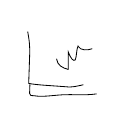
\begin{tikzpicture}[x={\dimexpr\dimen0/680\relax},y={\dimexpr-\dimen2/445\relax},line width=.3pt]
\path[use as bounding box] (0,0) rectangle (680,445);
\draw (0,25) .. controls (18,88) and (22,126) .. (20,170) -- (10,360) .. controls (80,370) and (220,374) .. (359,381) .. controls (433,390) and (502,375) .. (550,369);
\draw (22,367) -- (19,425) .. controls (17,443) and (38,437) .. (64,440) .. controls (145,449) and (237,438) .. (340,434) .. controls (463,430) and (561,439) .. (680,428);
\draw (285,201) .. controls (294,244) and (342,260) .. (402,270);
\draw (400,270) -- (401,157) .. controls (430,206) and (452,217) .. (469,209) .. controls (483,195) and (482,135) .. (497,119) .. controls (522,151) and (595,146) .. (638,136);
\end{tikzpicture}}}%
\kern4pt\box0\kern4pt\endgroup}

\uline{Corollaire} 1 Soient deux suites exactes
\diagram{\begin{tikzcd}[ampersand replacement=\&, column sep=small]
\cdot\arrow[r,no head]\&P'\arrow[r,no head]\&P\arrow[r,no head]\&P''\arrow[r,no head]\&\unsure{\cdot|0}\\
\cdot\arrow[r,no head]\&Q'\arrow[r,no head]\&Q\arrow[r]\&Q''\arrow[r]\&0
\end{tikzcd}}
et supposons que, pour un $\mathbb P$ de nbs premiers, on ait :
\[\unsure{\text{a}|\cdot})\quad p\in\mathbb P\Longrightarrow p\underline{P=P},\quad p\underline{Q'=Q'}\quad
\deleted{et\ pQ''=Q''\ \unsure{ou}\ \unsure{p\underline{P''=pP''}|p\underline{P''=P''}}}
\]
\inserted{(ou le symétrique)}
\margin{\begingroup
\setbox0=\hbox{\shortstack[l]{\deleted{(\unsure{donc} $pP=P$, $pQ=\unsure{0|Q}$)}\\[3ex]\strut}}
\dimen0=\wd0 \advance\dimen0 by 8pt
\dimen2=\ht0 \advance\dimen2 by \dp0 \advance\dimen2 by 8pt
\leavevmode\rlap{\raisebox{\dimexpr-\dp0-4pt\relax}{%
\begin{tikzpicture}[x={\dimexpr\dimen0/340\relax},y={\dimexpr-\dimen2/125\relax},line width=.3pt]
\path[use as bounding box] (0,0) rectangle (340,125);
\draw (-3,47)..controls (28,65) and (118,56)..(151,91)..controls (178,125) and (137,126)..(156,109)..controls (192,82) and (257,86)..(288,73);
\end{tikzpicture}}}%
\kern4pt\box0\kern4pt\endgroup}
\[
\text{b)}\quad\text{les.}\quad\varinjlim_{n\to\mathbb P}{}_nP\longrightarrow P''\quad\text{et}\quad
\underset{n\to\mathbb P}{\underline{\lim}}{}_nQ\mathbin{-}Q''\quad\text{épim.}
\]
\figure{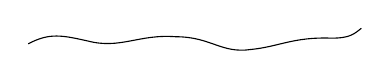
\begin{tikzpicture}[x=.018cm,y=-.018cm]
\draw (9,36) .. controls (24,28) and (33,30) .. (51,34) .. controls (74,40) and (87,29) .. (113,31) .. controls (138,31) and (145,43) .. (166,40) .. controls (186,38) and (196,31) .. (223,32) .. controls (236,32) and (239,29) .. (244,25);
\end{tikzpicture}}
\margin{\begingroup
\setbox0=\hbox{\parbox{.65\linewidth}{\unsure{Ne vaut que}, \unsure{celle en modules|cela ne marche} tel quel que si on suppose que $P',Q;P'',\unsure{G'|Q'|G.}$\\ \unsure{sont} $\mathbb P$ divisibles dans a), en plus de b).\\ Sinon, garder les ${}_nP\times{}_nQ\longrightarrow{}_nG\ \ldotp\ldotp\ldotp\ldotp\ldotp$}}
\dimen0=\wd0 \advance\dimen0 by 8pt
\dimen2=\ht0 \advance\dimen2 by \dp0 \advance\dimen2 by 8pt
\leavevmode\rlap{\raisebox{\dimexpr-\dp0-4pt\relax}{%
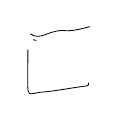
\begin{tikzpicture}[x={\dimexpr\dimen0/760\relax},y={\dimexpr-\dimen2/200\relax},line width=.3pt]
\path[use as bounding box] (0,0) rectangle (760,200);
\draw (30,18) .. controls (145,38) and (207,10) .. (382,8) .. controls (479,11) and (556,6) .. (686,-3);
\draw (2,64) .. controls (4,108) and (-5,166) .. (5,183) .. controls (13,199) and (69,190) .. (127,188) .. controls (318,184) and (495,174) .. (655,169) .. controls (670,169) and (674,166) .. (671,160);
\draw (59,35)--(96,37);
\end{tikzpicture}}}%
\kern4pt\box0\kern4pt\endgroup}

Alors le foncteur
\diagram{\begin{tikzcd}[ampersand replacement=\&]E\arrow[r,mapsto]\&(E',\varphi)\end{tikzcd}}
\unsure{associant à|associe à|envoyant} : \unsure{la|les} biext. de $P,Q$ par $G$ la restriction $E':P',Q'$ et la forme $\varphi_{E,\mathbb P}$
\diagram{\begin{tikzcd}[ampersand replacement=\&]\varphi:T_{\mathbb P}(P)\times T_{\mathbb P}(Q)\arrow[r,no head]\&T_{\mathbb P}(G)\end{tikzcd}}
prolongeant
\diagram{\begin{tikzcd}[ampersand replacement=\&]\varphi_{E',\mathbb P}:T_{\mathbb P}(P')\times T_{\mathbb P}(Q')\arrow[r,no head]\&T_{\mathbb P}(G)\end{tikzcd}}
est une équivalence de catégories.

\uline{Dém.} \inserted{\unsure{Supposons} p.ex.} On applique d'abord \begingroup
\setbox0=\hbox{\shortstack[l]{\hspace{1em}\deleted{\unsure{proposition}}\\le\quad corollaire 1 à}}
\dimen0=\wd0 \advance\dimen0 by 8pt
\dimen2=\ht0 \advance\dimen2 by \dp0 \advance\dimen2 by 8pt
\leavevmode\rlap{\raisebox{\dimexpr-\dp0-4pt\relax}{%
\begin{tikzpicture}[x={\dimexpr\dimen0/530\relax},y={\dimexpr-\dimen2/190\relax},line width=.3pt]
\path[use as bounding box] (0,0) rectangle (530,190);
\draw (98,136)..controls (80,110) and (120,86)..(166,86)..controls (230,82) and (291,75)..(294,68);
\end{tikzpicture}}}%
\kern4pt\box0\kern4pt\endgroup
\diagram{\begin{tikzcd}[ampersand replacement=\&, column sep=small]0\arrow[r,no head]\&P'\arrow[r]\&P\arrow[r,no head]\&P''\arrow[r,no head]\&\unsure{\cdot|0}\end{tikzcd}}
et $Q'$, en utilisant $pQ'=Q'$, $\underset{\unsure{\longrightarrow|\mathbin{-}}}{\lim}{}_nP\longrightarrow P''$ épim.

Cela donne une description des biextensions de $P,Q'$. On applique ensuite le sym. du cor. 1 à $P$ et
\diagram{\begin{tikzcd}[ampersand replacement=\&, column sep=small]\unsure{\cdot|0}\arrow[r]\&Q'\arrow[r]\&Q\arrow[r]\&Q''\arrow[r]\&0,\end{tikzcd}}
en utilisant $pP=P$ \begingroup
\setbox0=\hbox{\deleted{\unsure{i.e.|et} $\unsure{pP''=P''}$}}
\dimen0=\wd0 \advance\dimen0 by 8pt
\dimen2=\ht0 \advance\dimen2 by \dp0 \advance\dimen2 by 8pt
\leavevmode\rlap{\raisebox{\dimexpr-\dp0-4pt\relax}{%
\begin{tikzpicture}[x={\dimexpr\dimen0/270\relax},y={\dimexpr-\dimen2/125\relax},line width=.3pt]
\path[use as bounding box] (0,0) rectangle (270,125);
\draw (61,58) -- (60,48) .. controls (102,61) and (142,42) .. (216,43) -- (217,38);
\end{tikzpicture}}}%
\kern4pt\box0\kern4pt\endgroup et $\varinjlim_{n\to\mathbb P}{}_nQ\mathbin{-}Q''$ épim.
\margin{49}
